\section{Results and Analysis}
\label{sec:results}
\subsection{Experimental Setup}
\kechen{I have a slight concern about the scalability of this approach, both with varying beam size and number of labels. I'm curious about the computational complexities of the training and prediction methods provided in the Algorithm 2 and Algorithm 3 and how that compares with existing methods.}
We test our proposed set-RNN method on 4 real-world datasets, RCV1-v2, Slashdot, TheGuardian, and Arxiv Academic Paper Dataset (AAPD) \cite{DBLP:journals/corr/abs-1806-04822}. We take the public RCV1-v2 release\footnote{\scriptsize\url{http://www.ai.mit.edu/projects/jmlr/papers/volume5/lewis04a/lyrl2004_rcv1v2_README.htm}} and randomly sample 50,000 documents. We crawl Slashdot and TheGuardian documents from their websites\footnote{\scriptsize Slashdot: \url{https://slashdot.org/} Note that there is another public Slashdot multi-label dataset \cite{read2009classifier} but we do not use that one because it is quite small. TheGuardian: \url{https://www.theguardian.com}  
} and treat the official editor tags as ground truth. We also gather a list of user tags\footnote{\scriptsize \url{www.zubiaga.org/datasets/socialbm0311/}} for each document and treat them as additional features. For AAPD dataset, we follow the same train/test split as in \cite{DBLP:journals/corr/abs-1806-04822}. Table \ref{tab:stats} contains statistics of these four datasets. 
\begin{table}[h]
	\resizebox{1.01\columnwidth}{!}{%resize the table
\begin{tabular}{|l|c|c|c|c|c|c|}
  \hline
  Data & \#train & \#test & cardinality & \#labels & doc length  \\
  \hline
  Slashdot & 19,258 & 4,814& 4.15& 291&64 \\
  RCV1-v2 & 40,000& 10,000&  3.17& 101&121 \\
  TheGuardian & 37,638 & 9,409 & 7.41& 1,527&505 \\
  AAPD & 53,840 & 1,000 & 2.41& 54 & 163 \\
  \hline
\end{tabular}
}
\caption{\fontsize{10}{12}\selectfont  Statistics of the datasets.}\label{tab:stats}
\end{table}


\begin{table*}[ht]
	\begin{center}
	\resizebox{2.1\columnwidth}{!}{%resize the table
		\begin{tabular}{|l|cc|cc|cc|cccc|}
			\hline
			\multirow{2}{*}{Methods}	&  
             \multicolumn{2}{c|}{Slashdot}&\multicolumn{2}{c|}{RCV1-v2}&\multicolumn{2}{c|}{TheGuardian}&\multicolumn{4}{c|}{AAPD} \\
             \cline{2-11}
           & label-F1 & instance-F1  & label-F1 & instance-F1 & label-F1 & instance-F1 & label-F1 & instance-F1 & Hamming-Loss & Micro-F1 \\

                        \hline
            BR
            & .271 & .484 & .486 & .802 &.292 & .572 & .529 & .654 & .0230 & .685 \\
            BR-support
            & .247 & .516 & .486 & .805 &.296 & .594 & .545 & .689 & \textbf{.0228} & .696\\
            PCC 
            & .279 & .480 & .595 & .818 &- & - & .541 & .688 & .0255 & .682 \\
            seq2seq-RNN  
             & .270 & .528 & .561 & .824 &.331 & .603 & .510 & .708 & .0254 & .701 \\
            Vinyals-RNN-uniform 
             & .279 & .527 & .578 & .826 & .313 & .567  & .532 & .721 & .0241 & .711\\
            Vinyals-RNN-sample
            & .300 & .531 & .590 & .828 & .339 & .597 &-&-&-&-\\
            Vinyals-RNN-max
            & .293 & .530 & .588 & .829 & .343 & .599 & .535 & .709 & .0256 & .700 \\
            Vinyals-RNN-max-direct
             & .226 & .518 & .539 & .808 & .313 & .583 &-&-&-&-\\
            SGM
            &-&-&-&-&-&-& - & - & .0245 & .710 \\
            set-RNN 
             & \textbf{.310} & \textbf{.538} & \textbf{.607} & \textbf{.838}  &\textbf{.361} & \textbf{.607} & \textbf{.548} & \textbf{.731} & .0241 & \textbf{.720}\\
            \hline

		\end{tabular}
		}
	\end{center}
	\caption{Comparison of different approaches. ``-'' means result not available. For \emph{hamming loss}, the lower the value is, the better the model performs. For all other measures, the higher the better.%\kechen{cardinality analysis, V's method can't perform well on Guardian. why?}
    }\label{tab:main}
\end{table*}





\begin{table*}[ht]
  \begin{center}
  	\resizebox{2.1\columnwidth}{!}{%resize the table

    \begin{tabular}{|l|cc|cc|cc|cc|}
      \hline
      \multirow{2}{*}{Methods}  &  
             \multicolumn{2}{c|}{Slashdot}&\multicolumn{2}{c|}{RCV1-v2}&\multicolumn{2}{c|}{TheGuardian}&\multicolumn{2}{c|}{AAPD} \\
             \cline{2-9}
           & label-F1 & instance-F1  & label-F1 & instance-F1 & label-F1 & instance-F1 & label-F1 & instance-F1\\

                        \hline
            seq2seq-RNN  
             & .270$\to$.269 & .528$\to$.528& .561$\to$.561 & .824$\to$.824 &.331$\to$.336& .603$\to$.603 & .510$\to$.511 &.708$\to$.709 \\
            Vinyals-RNN-uniform  
             & .279$\to$.288& \textbf{.527}$\to$\textbf{.537}& .578$\to$.587& .826$\to$.833& \textbf{.313}$\to$\textbf{.336}& \textbf{.567}$\to$\textbf{.585} & \textbf{.532}$\to$\textbf{.542} &.721$\to$.724 \\
             Vinyals-RNN-sample
            & .300$\to$.303 & .531$\to$.537 &.590$\to$.597 & .828$\to$.833 & \textbf{.339}$\to$\textbf{.351} & .597$\to$.602 & - &- \\
            Vinyals-RNN-max
            & .293$\to$.301 & .530$\to$.535 & .588$\to$.585 & .829$\to$.830 & .343$\to$.352 &.599$\to$.604 & .535$\to$.537 &.709$\to$.712  \\
            Vinyals-RNN-max-direct
             & .226$\to$.228& .518$\to$.519& .539$\to$.538& .808$\to$.808& .313$\to$.316&.583$\to$.584 & - &- \\
            
            set-RNN 
             & \textbf{.297}$\to$\textbf{.310} & \textbf{.528}$\to$\textbf{.538} & \textbf{.593}$\to$\textbf{.607} & .831$\to$.838 &\textbf{.349}$\to$\textbf{.361} & \textbf{.595}$\to$\textbf{.607} & .548$\to$.548 &.728$\to$.731 \\\hline

    \end{tabular}
    }
  \end{center}
  \caption{Predicting the most probable sequence vs. predicting the most probable set. Numbers before the arrow: predicting the most probable sequence. Numbers after the arrow: predicting the most probable set. We highlight scores which get significantly improved in \textbf{bold} (improvement is larger than 0.01).
    }\label{table_prediction}
\end{table*}

 To process documents, we filter out stopwords and punctuations. Each document is truncated to have maximum 500 words for TheGuardian and AAPD, and 120 for Slashdot and RCV1-v2. Numbers and out-of-vocabulary words are replaced with special tokens. Words, user tags and labels are all encoded as 300-dimensional vectors using \textsc{word2vec} \cite{DBLP:journals/corr/abs-1301-3781}.
 
 We implement  RNN with attention using \textsc{tensorflow-1.4.0} \cite{DBLP:conf/osdi/AbadiBCCDDDGIIK16}. The dynamic function for  RNNs is chosen to be Gated recurrent units (GRU) with  2 layers and at most 50 units in decoder. The  size of the GRU unit is 300. We set dropout rate to 0.3, and train the model with Adam optimizer \cite{DBLP:journals/corr/KingmaB14} with learning rate $0.0005$. Beam size is set to be 12 at both training and inference stages. We adopt \emph{label-F1} (average F1 over labels) and \emph{instance-F1} (average F1 over instances) as our main evaluation metrics, as defined below:
 
\begin{align*} \text{label-F1} = \frac{1}{L}\sum_{\ell=1}^L\frac{2\sum_{n=1}^N y^{(n)}_\ell \hat{y}^{(n)}_\ell}{\sum_{n=1}^N y^{(n)}_\ell+\sum_{n=1}^N \hat{y}^{(n)}_\ell}\\
\text{instance-F1} = \frac{1}{N}\sum_{n=1}^N\frac{2\sum_{\ell=1}^L y^{(n)}_\ell \hat{y}^{(n)}_\ell}{\sum_{\ell=1}^L y^{(n)}_\ell+\sum_{\ell=1}^L \hat{y}^{(n)}_\ell}
\end{align*}
where for each instance $n$, $y_\ell^{(n)}=1$ if label $\ell$ is a given label in ground truth; $\hat{y}_\ell^{(n)}=1$ if label $\ell$ is a predicted  label.

We compare our method with the following methods: 
\begin{itemize}
	\item \textbf{Binary Relevance (BR)} \cite{tsoumakas2007multi} with both independent training and prediction;
	\item \textbf{Binary Relevance with support inference (BR-support)} \cite{wang2017regularizing} which trains binary classifiers independently but imposes label constraints at prediction time by only considering label sets observed during training, namely $\hat{\mathbf{y}}=\arg\max_{\text{observed~}\mathbf{y}}\prod_{\ell=1}^L p(y_{\ell}|x)$;
	\item \textbf{Probabilistic Classifier Chain (PCC)} \cite{DBLP:conf/icml/DembczynskiCH10} which transforms the multi-label classification task into a chain of binary classification problems.
    \item \textbf{Sequence to Sequence RNN (seq2seq-RNN)} \cite{DBLP:conf/nips/NamMKF17} which maps each set to a sequence by decreasing label frequency and solves the multi-label task with an RNN designed for sequence prediction (see Table \ref{tab_objs}). 
    \item \textbf{Vinyals-RNN-uniform, Vinyals-RNN-sample, and Vinyals-RNN-max} are three variants of RNNs proposed by \cite{vinyals2015order}. They are trained  with different objectives that correspond to different transformations between sets and sequences. See Table~\ref{tab_objs} for a summary of their training objectives. Following the approach taken by \cite{vinyals2015order}, Vinyals-RNN-sample and Vinyals-RNN-max are initialized by Vinyals-RNN-uniform. We have also tested training Vinyals-RNN-max directly without having Vinyals-RNN-uniform as an initialization, and we name it as  \textbf{Vinyals-RNN-max-direct}.
    \item \textbf{Sequence Generation Model (SGM)} \cite{DBLP:journals/corr/abs-1806-04822} which trains the RNN model similar to seq2seq-RNN but uses a new decoder structure that computes a weighted global embedding based on all labels as opposed to just the top one at each time step.
\end{itemize}

In BR and PCC, logistic regressions with L1 and L2 regularizations are used as the underlying binary classifiers. seq2seq-RNN, PCC, and SGM rely on a particular label order. We adopt the decreasing label frequency order, which is the most popular choice.

%Additionally in order to measure the effect of summing up sequence probabilities at prediction time, we test a variant of seq2seq RNN (named seq2seq RNN w/ set pred) which sums up sequence probabilities during prediction, and a variant of our proposed method (named set-RNN w/o set pred) which only predicts the most probable sequence.

% For fixed ordering experiments, we keep the order of both input and output, which means we are using a sequence-to-sequence (seq2seq) \cite{DBLP:conf/nips/SutskeverVL14}. To be specific, we represent the document as a sequence of words, then sort the output labels based on count of occurrences in descending order. This setup is the same as \newcite{DBLP:conf/nips/NamMKF17}'s work,  that's why we call it \textsc{fix\_order\_Nam}. For non fixed ordering experiments, in contrary to ordered sequences, we represent the document as a bag of words and feed the labels into the model as a set. We set beam width 12 and 6 in two-level beam search, which means we select top 12 sequences based on sequence probability and rerank them with their set probability based on top 6 permutations. We name our model \textsc{blabla}.

% \textbf{Results.}

\subsection{Experimental Results}

Table \ref{tab:main} shows the performance of different methods in terms of \emph{label-F1} and \emph{instance-F1}. The SGM results are taken directly from \cite{DBLP:journals/corr/abs-1806-04822}, and are originally reported only on AAPD dataset in terms of Hamming-Loss and Micro-F1. Definitions of these two metrics can be found in \cite{koyejo2015consistent}.  
% The second best method is the variant of our method without the sequence probability summation at prediction. Comparing these two, we can see the benefit of summing up sequence probabilities at prediction time (the beam search for summation step does not add much computation). 

 
Our method performs the best in all metrics on all datasets. All RNN based methods perform better than traditional methods BR, BR-support and PCC. Among the Vinyals-RNN variants, Vinyals-RNN-max and Vinyals-sample work the best and have similar performance. However, they have to be initialized by Vinyals-RNN-uniform. Otherwise, the training gets stuck in early stage and the performance degrades significantly. One can see the clear degradation by comparing the Vinyals-RNN-max row (with initialization) with the Vinyals-RNN-max-direct row (without initialization). By contrast, our training objective in set-RNN does not suffer from this issue and can serve as a stable stand alone training objective.

\begin{figure}[t]
%\hspace{-2ex}
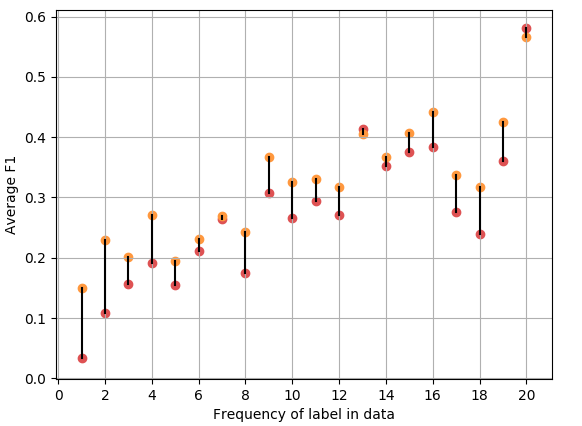
\includegraphics[width=1.0\columnwidth]{figs/labelf1.png}

\caption{Average F1 over rare labels with the same frequency on TheGuardian dataset. Orange=set-RNN, Red=seq2seq-RNN.}
\label{fig:labelf1}
%\vspace{-6ex}
\end{figure}

On TheGuardian dataset, set-RNN performs slightly better than seq2seq-RNN in terms of instance-F1, but much better in terms of label-F1. It is known that instance-F1 is basically determined by the popular labels' performance while label-F1 is also sensitive to the performance on rare labels. Figure~\ref{fig:labelf1} shows that set-RNN predicts rare labels better than seq2seq-RNN.

Next we analyze how much benefit our new set prediction strategy brings in. For each RNN-based method, we test two prediction strategies: 1) finding the sequence with the highest probability and outputting the corresponding set (this is the default prediction strategy for all models except set-RNN); 2) outputting the set with the \kechen{approximated} highest probability (this is the default prediction strategy for set-RNN). Table~\ref{table_prediction} shows how each method performs with these two prediction strategies. One can see that Vinyals-RNN-uniform and set-RNN benefit most from predicting the top set,  Vinyals-RNN-sample, Vinyals-RNN-max and Vinyals-RNN-max-direct benefit less, and seq2seq RNN does not benefit at all. Intuitively, for the top-set prediction to be different from the top-sequence prediction, the model has to spread probability mass across different sequence permutations of the same set. 

This motivates us to check how sharply (or uniformly) distributed the probabilities are over different sequence permutations of the predicted set. We first normalize these sequence probabilities related to the predicted set and then compute the entropy. To make predictions with different set sizes (and hence different number of sequence permutations) comparable, we further divide the entropy by the logarithm of number of sequences. Smaller entropy values indicate a sharper distributions. The results are shown in Figure~\ref{fig:entropy}.

seq2seq-RNN trained with fixed label order and standard RNN objective (\ref{eq:standard_rnn}) generates very sharp sequence distributions. It basically only assigns probability to one sequence in the given order. The entropy is close to 0. In this case, predicting the set is no different than predicting the top sequence (see Table~\ref{table_prediction}). On the other extreme is Vinyals-RNN-uniform, trained with objective (\ref{eq:wrong_obj}), which spreads probabilities across many sequences, and leads to the highest entropy among all models tested (the uniform distribution has the max entropy of 1). From Table~\ref{table_prediction}, we see that by summing up sequence probabilities and predicting the most probable set,  Vinyals-RNN-uniform's performance  improves. But as  discussed earlier, training with the objective (\ref{eq:wrong_obj}) makes it impossible for the model to discover and concentrate on a particular natural label order (represented by a sequence). Overall Vinyals-RNN-uniform is not competitive even with the set-prediction enhancement. Between the above two extremes are Vinyals-RNN-max and set-RNN (we have omitted Vinyals-RNN-sample and Vinyals-RNN-max-direct here as they are similar to Vinyals-RNN-max). Both models are allowed to assign probability mass to a subset of sequences. Vinyals-RNN-max produces sharper sequence distributions than set-RNN, because  Vinyals-RNN-max has the incentive to allocate most of the probability mass to the most probable sequence due to the max operator in its training objective (\ref{eq:max_obj}). From Table~\ref{table_prediction}, one can see that set-RNN clearly benefits from summing up sequence probabilities and predicting the most probable set while Vinyals-RNN-max does not benefit much. Therefore, the sequence probability summation is best used in both training and prediction, as in our proposed method.

Comparing 4 datasets in Table~\ref{table_prediction}, we also see that Slashdot and TheGuardian, which have larger label cardinalities (therefore more permutations for one set potentially), benefit more from predicting the most probable set than RCV1 and AAPD, which have smaller label cardinalities.

% By design, Vinyals-RNN-uniform and set-RNN could spread probabilities mass across many sequence permutations of the same set, Vinyals-RNN-sample, Vinyals-RNN-max and Vinyals-RNN-max-direct tends to allocate most of the probability mass to the top sequence, and seq2seq basically only assigns probability to the sequence in the given order. 

% To further validate our intuition, 


% seq2seq-RNN performs better than traditional methods BR, BR w/support and PCC. Adding set probability summation at prediction time does not further improve its performance. We suspect that since the model is trained to respect the given label order (decreasing label frequency order in this case), at prediction time, only sequences (roughly) in that order receives decent probabilities. Therefore the set probability is basically determined by the top sequence. Thus the sequence probability summation is best used in both training and prediction, as in our proposed method.


% (1) We can see that Vinyal\_final performs much better than Vinyal\_final\_noinit, which shows evidence to support our hypothesis that objective \ref{eq:max_obj} have to be initialized by a model pretrained with objective \ref{eq:wrong_obj}. Compare Vinyal- 

% (2) Vinyal\_final outperforms seq2seq RNN in Slashdot and RCV-v2, but not in TheGuardian. When cardinality is large, Vinyal's method can easily get stuck on bad prediction (and reinforce it). Comparing with Vinyal's method, our method is more stable and performs well in all three data sets.

% (3) Adding set prediction helps in both Vinyal's and our methods. \kechen{(1) difference between sample and max (2) labelF1 and InstanceF1 (3) highlight in table 4.}

\begin{figure}[t]
%\hspace{-2ex}
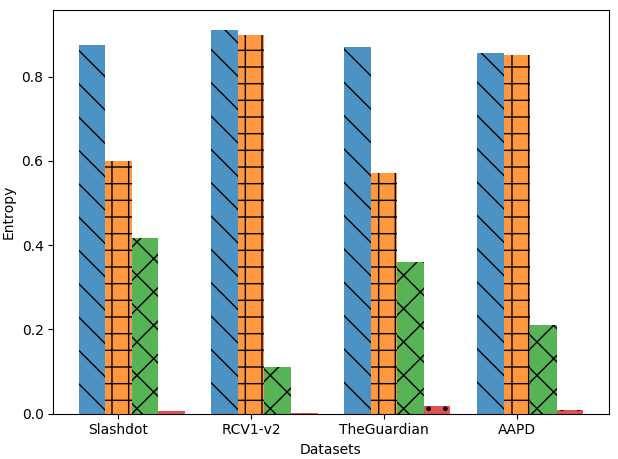
\includegraphics[width=1.00\columnwidth]{figs/entropy.png}

\caption{Entropy of sequence probability distribution for each model. Blue(\textbackslash)=Vinyals-RNN-uniform, Orange(+)=set-RNN, Green($\times$)=Vinyals-RNN-max, Red($\cdot$)=seq2seq-RNN.}
\label{fig:entropy}
%\vspace{-6ex}
\end{figure}


% \textbf{Entropy Analysis} We normalize the probabilities of top probable sequences inferred via different decoding algorithms, and compute entropy of the normalized probability distribution. The experimental result shows how different methods, which correspond to different objectives, generate different shapes of sequence distribution. The smaller entropy indicates sharper sequence probability distribution.

% (1) Training with standard RNN objective (objective \ref{eq:standard_rnn}) generates very sharp sequence probability distribution. 

% (2) Similar to RNN objective, Vinyal\_final (objective \ref{eq:max_obj}) maximizes the probability of the top sequence prediction, with additional ability to train on changing top prediction. This is why it is less sharper than RNN. The model assign the top sequence prediction a large probability, while probabilities of other predictions are very small.

% (3) Vinyal\_init is trying to optimize product of sequence probability (objective \ref{eq:wrong_obj}). Having avoided negative influence from exceptionally small probability, the model assign these predictions relatively uniform probabilities (the biggest entropy).

% (4) The entropy of our method (objective \ref{eq:right_obj}) is in the middle between vinit and vfinal. It demonstrates that our model assign relatively large probability to multiple sequences.




  % \begin{figure*}[ht]

  % \begin{minipage}{.5\linewidth}
  % \centering
  % \subfloat[]{\label{main:a}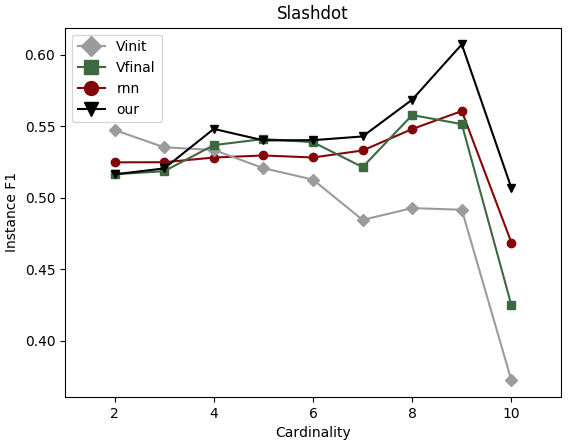
\includegraphics[scale=.35]{figs/slash.png}}
  % \end{minipage}%
  % \begin{minipage}{.5\linewidth}
  % \centering
  % \subfloat[]{\label{main:b}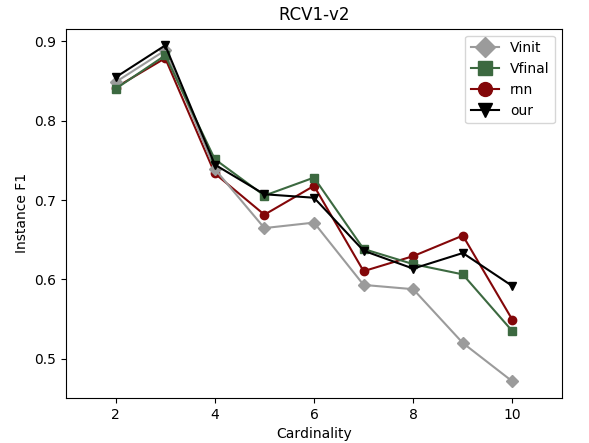
\includegraphics[scale=.35]{figs/reuter.png}}
  % \end{minipage}\par\medskip
  % \centering
  % \subfloat[]{\label{main:c}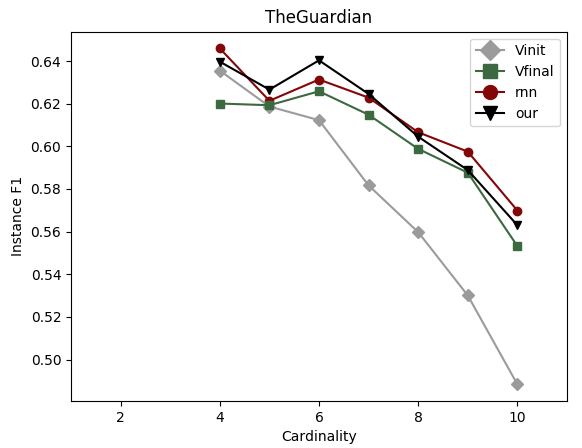
\includegraphics[scale=.35]{figs/guardian.png}}

  % \caption{Performance of different models on different cardinality subset}
  % \label{fig:main}
  % \end{figure*}


% \textbf{Cardinality Analysis} We group documents with the same cardinality into different subsets and individually present instance F1 on each subset. 

% (1) The performance of Vinyal\_init drops a lot as the cardinality increases.

% (2) The performance of our method scales well with cardinality. It outperforms other methods when cardiality is large.

% (3) 